\documentclass[tikz,border=3pt]{standalone}
\usepackage[utf8]{inputenc}
\usepackage[T1]{fontenc}
\usepackage{libertinus}
\usepackage{amsmath,amssymb}
\usetikzlibrary{arrows.meta,calc,patterns,decorations.pathmorphing,decorations.markings,decorations.pathreplacing,bending}
\definecolor{UGblue}{RGB}{0,51,102}
\newcommand{\dbar}{\mathchar'26\mkern-12mu d}
\tikzset{
  >=Stealth,
  every node/.style={font=\small},
  caja/.style={draw,line width=0.9pt},
  pared/.style={draw,line width=1.6pt},
  ejes/.style={->,line width=0.8pt},
  adia/.style={draw,pattern=north east lines,pattern color=black!70,line width=0.5pt},
  gas/.style={fill=UGblue!8},
  punto/.style={fill,circle,inner sep=1.3pt},
  onda/.style={decorate,decoration={snake,amplitude=1.1pt,segment length=5pt,post length=3pt,pre length=0pt}},
}
\begin{document}
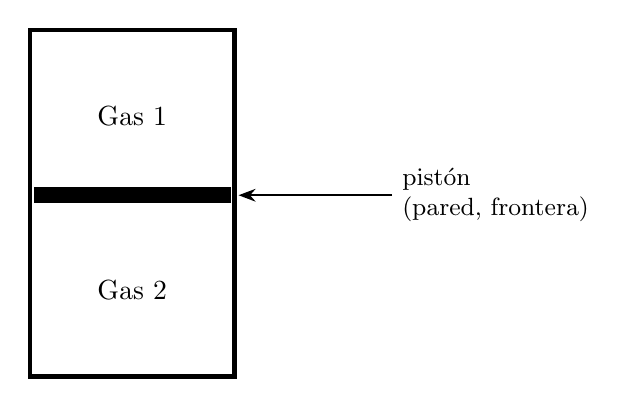
\begin{tikzpicture}
  \draw[pared] (0,0) -- (0,4.4) -- (2.6,4.4) -- (2.6,0) -- cycle;
  \fill[black] (0.05,2.2) rectangle (2.55,2.4);
  \node at (1.3,3.3) {\normalsize Gas 1};
  \node at (1.3,1.1) {\normalsize Gas 2};
  \draw[->,line width=0.7pt] (4.6,2.3) node[right,align=left] {pistón\\(pared, frontera)} -- (2.65,2.3);
\end{tikzpicture}
\end{document}
